\documentclass{article}

\usepackage[education,final]{neurips_2026}

\usepackage[utf8]{inputenc}
\usepackage[T1]{fontenc}
\usepackage{hyperref}
\usepackage{url}
\usepackage{booktabs}
\usepackage{amsfonts}
\usepackage{nicefrac}
\usepackage{microtype}
\usepackage{xcolor}
\usepackage{graphicx}
\usepackage{tcolorbox}
\usepackage{enumitem}
\usepackage{float}
\setlist{noitemsep, topsep=2pt, parsep=0pt, partopsep=0pt, leftmargin=1.4em}
% tighten the space floats claim above/below themselves and around their captions
\setlength{\intextsep}{5pt plus 1pt minus 1pt}
\setlength{\textfloatsep}{5pt plus 1pt minus 1pt}
\setlength{\abovecaptionskip}{4pt}
\setlength{\belowcaptionskip}{0pt}

\newcommand{\minidogicon}{\raisebox{-0.22em}{
\includegraphics[height=1.05em]{figs/icon_minidog.png}}}

\title{\minidogicon\, MiniDog: \\
Dog-Breed Text-to-Image Diffusion, from Pretraining \\
to Fine-Tuning, on 4 Consumer GPUs}

\author{%
  Reyhaneh Esmailizadeh \quad Xingjian Leng \quad Zhanhao Liang \quad Liang Zheng \\
  Australian National University \\
  {\small\texttt{\{reyhaneh.esmailizadeh, xingjian.leng, zhanhao.liang, liang.zheng\}@anu.edu.au}}
}

\begin{document}
\raggedbottom

\maketitle
\vspace{-2.2em}

\textbf{Abstract}. Training diffusion transformers (DiTs) is usually presented as something that requires
industrial-scale compute, and thus has very little, if any, empirical exercise for student learning despite its vital significance in the AI industry. To fill this gap, this resource provides a runnable pipeline which pretrains a working text-to-image DiT to an FID below 10 in just 2.5 hours, and fine-tunes it in 20 more minutes, on hardware any student can rent with \$3-\$5 expense. The recipe follows from a systematic comparison of image tokenizers, representation-alignment losses, and text token budgets. No pretrained weights are used. Students will be able to run the recipe to do training, evaluation, and visualization themselves. Code, configs, model weights, and the full tutorial notebook are provided at \url{https://github.com/Reyhaneesmailizadeh/diffusion-bench}.

\begin{tcolorbox}[colback=green!5!white, colframe=green!35!black, boxrule=0.6pt, arc=1mm,
  left=5pt, right=5pt, top=3pt, bottom=3pt]
\textbf{2h50m total training on 4$\times$RTX~3090 (24GB) $\rightarrow$ \$3--\$5 of rented compute $\rightarrow$ FID = 9.4} \\
2.5h pretrain (Task~2, Exp.~1) + 20min fine-tune (Task~2, Exp.~2). GPU pricing: Vast.ai
\$0.25/GPU/hr, RunPod \$0.46/GPU/hr.
\end{tcolorbox}

\vspace{-0.4em}
\begin{figure}[H]
  \centering
  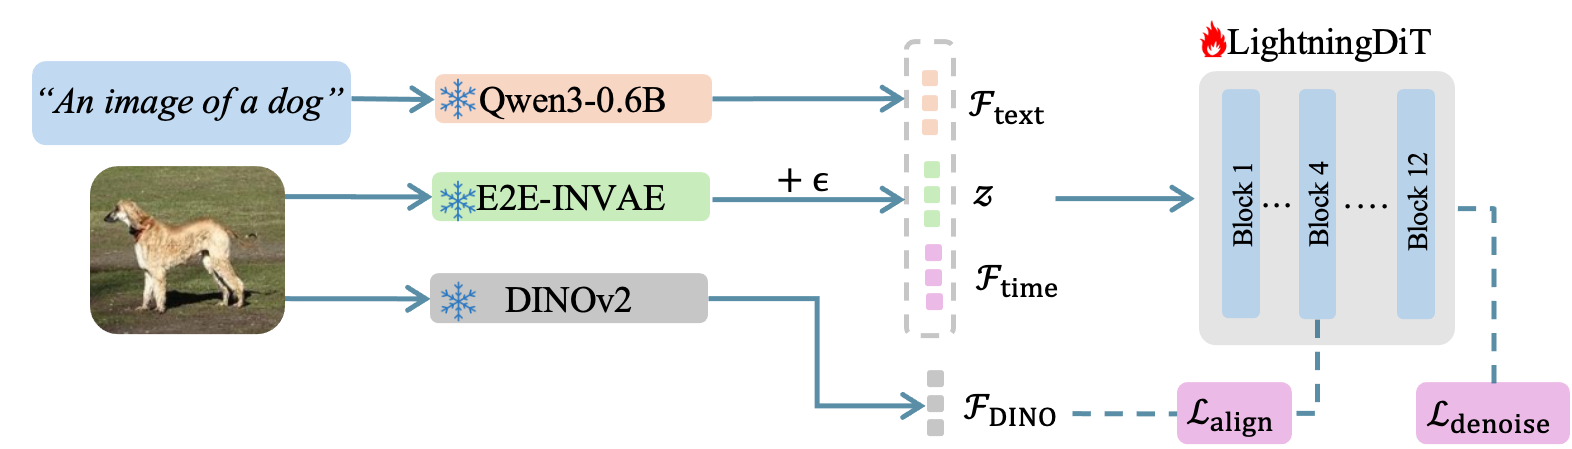
\includegraphics[width=0.82\linewidth]{figs/Picture 1.png}
  \vspace{-0.5em}
  \caption{Training architecture (\raisebox{-0.15em}{
\includegraphics[height=0.9em]{figs/icon_snowflake.png}} = frozen, \raisebox{-0.15em}{
\includegraphics[height=0.9em]{figs/icon_flame_white.png}} = trained).}
\end{figure}

\vspace{-0.6em}
\paragraph{Learning objectives}
\begin{itemize}
  \item Understand latent diffusion and derive the flow-matching training objective [1].
  \item Compare in-context (token-based) conditioning to AdaLN-Zero [2], and apply
    REPA-style auxiliary losses [4] that align internal DiT features with a pretrained encoder (DINOv2 [5]).
  \item See how tokenizer/training recipe choices determine whether DiT training is
    affordable on consumer GPUs. Build a full data $\to$ precompute pipeline.
  \item Diagnose what the fine-tuning FID curve measures, and score generations with
    learned human-preference models (PickScore [6], HPSv2 [7]).
\end{itemize}

\vspace{-0.2em}
\paragraph{Task 1: Diffusion basics.} The accompanying notebook opens with a self-contained study on toy data, where students reproduce a recent finding that flow-matching models predicting clean data ($x$-prediction) scale cleanly to high ambient dimension while those predicting velocity ($v$-prediction) degrade unless given substantially more model capacity. Students verify this directly: training all four prediction/loss combinations across three toy datasets and three ambient dimensions, then testing whether scaling model capacity can rescue $v$-prediction, and finally implementing MeanFlow for one-step generation. This distinguishes the failure as data-dependent rather than universal. Our DiT operates on a 32-channel latent whose intrinsic dimensionality is far higher than the toy manifolds, motivating our use of $v$-prediction in the full pipeline that follows.

\paragraph{Task 2: Training a text-to-image DiT end to end.} The remainder of the resource builds the full pipeline. The notebook (13 sections) ties background
theory to training code, runs each model component individually (VAE tokenizer, text encoder (Qwen3 [8]), REPA target, the DiT backbone), builds the data pipeline, runs pretraining and
fine-tuning with classifier-free guidance [3], and evaluates with FID/IS and learned human-preference models. The backbone is LightningDiT [10] over the end-to-end tuned E2E-INVAE tokenizer [9], and all experiments are run within the DiffusionBench framework [11]. Every code cell
is real, executable code from the actual research codebase, not a simplified
reimplementation.

\paragraph{Data.} Pretraining uses 26000 recaptioned dog images spanning 20 breeds; SFT uses a smaller, cleaner set of 2000 Flux.1-generated synthetic images over the same 20 breeds; reward-model evaluation uses a held-out set of 500 captions. All three are hosted on Hugging Face (\texttt{reyhanehesi/dog-t2i-diffusion-data}).

\vspace{0.1em}
{We show example training curves below using pretraining. Students are asked to reproduce and diagnose the results in Sections 10 and 12
of the notebook.}

\begin{figure}[H]
  \centering
  \vspace{-0.3em}
  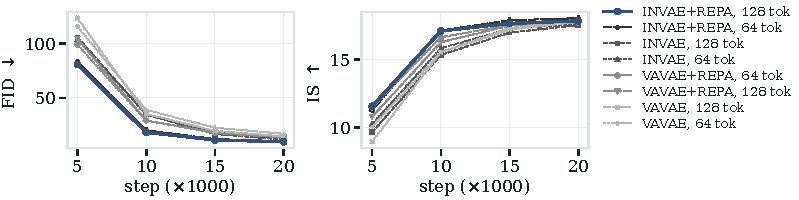
\includegraphics{figs/experiment_plots_row.pdf}
  \vspace{-0.5em}
  \caption{\textbf{Pretraining} across tokenizer, REPA, and token-budget settings (200 epochs each).
    Our best run (blue), E2E-INVAE [9] with REPA [4] at 128 tokens, reaches FID 9.4 / IS 17.9; grey
    curves are the other seven variants (best FID 9.8). Labels without ``+REPA'' omit the alignment loss.}
\end{figure}

\vspace{-0.4em}
\paragraph{Reward model evaluation.} Evaluating pre-trained and SFT models using reward models. We use HPSv2 and PickScore, both trained with human evaluation results. HPSv2 scores each image, and we report the average score over 500 generated images. PickScore uses two images as input and outputs the probability of it being referred over the other; 500 image pairs are used. We clearly observe that the SFT model is superior to the pretrained model.

\begin{figure}[H]
  \centering
  \begin{minipage}[c]{0.30\linewidth}
    \centering
    \footnotesize
    \setlength{\tabcolsep}{3.5pt}
    \begin{tabular}{lcc}
      \toprule
                 & HPSv2  & PickScore \\
      \midrule
      Pretrained & 0.2406 & 2.2\%  \\
      SFT        & 0.2713 & 97.8\% \\
      \bottomrule
    \end{tabular}
  \end{minipage}\hfill
  \begin{minipage}[c]{0.35\linewidth}
    \centering
    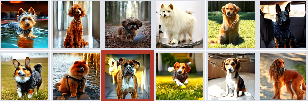
\includegraphics[width=\linewidth]{figs/sft_samples_grid_2x6.pdf}
  \end{minipage}\hfill
  \begin{minipage}[c]{0.32\linewidth}
    \begin{tcolorbox}[colback=black!3!white, colframe=black!25!white, boxrule=0.4pt,
      arc=0.6mm, left=3pt, right=3pt, top=2pt, bottom=2pt]
      \scriptsize
      ``Boxer with a wet brindle with white markings coat twists mid-shake on a sheltered wooden porch, droplets flinging from its short fur and loose jowls.''\,\dots
    \end{tcolorbox}
  \end{minipage}
  \vspace{-0.3em}
  \caption{Reward-model scores (left), 12 sample generations from the SFT model (middle), and
    the opening of the text prompt for the highlighted sample (right). Remaining prompts are provided in the notebook.}
\end{figure}

\vspace{-0.9em}
\section*{References}
\vspace{-0.5em}
{\footnotesize
\begin{itemize}[leftmargin=1.9em, label={}, itemsep=0pt, topsep=1pt]
  \item[{[1]}] Lipman, Y.\ et al.\ (2022) Flow matching for generative modeling. \href{https://arxiv.org/abs/2210.02747}{arXiv:2210.02747}.
  \item[{[2]}] Peebles, W.\ \& Xie, S.\ (2022) Scalable diffusion models with transformers (DiT). \href{https://arxiv.org/abs/2212.09748}{arXiv:2212.09748}.
  \item[{[3]}] Ho, J.\ \& Salimans, T.\ (2022) Classifier-free diffusion guidance. \href{https://arxiv.org/abs/2207.12598}{arXiv:2207.12598}.
  \item[{[4]}] Yu, S.\ et al.\ (2024) Representation alignment for generation: training diffusion transformers is easier than you think (REPA). \href{https://arxiv.org/abs/2410.06940}{arXiv:2410.06940}.
  \item[{[5]}] Oquab, M.\ et al.\ (2023) DINOv2: learning robust visual features without supervision. \href{https://arxiv.org/abs/2304.07193}{arXiv:2304.07193}.
  \item[{[6]}] Kirstain, Y.\ et al.\ (2023) Pick-a-Pic: an open dataset of user preferences for text-to-image generation (PickScore). \href{https://arxiv.org/abs/2305.01569}{arXiv:2305.01569}.
  \item[{[7]}] Wu, X.\ et al.\ (2023) Human preference score v2: a solid benchmark for evaluating human preferences of text-to-image synthesis. \href{https://arxiv.org/abs/2306.09341}{arXiv:2306.09341}.
  \item[{[8]}] Qwen Team (2025) Qwen3 technical report. \href{https://arxiv.org/abs/2505.09388}{arXiv:2505.09388}.
  \item[{[9]}] Leng, X.\ et al.\ (2025) REPA-E: unlocking VAE for end-to-end tuning with latent diffusion transformers. \emph{ICCV 2025}. \href{https://arxiv.org/abs/2504.10483}{arXiv:2504.10483}.
  \item[{[10]}] Yao, J.\ et al.\ (2025) Reconstruction vs.\ generation: taming optimization dilemma in latent diffusion models (VA-VAE and LightningDiT). \emph{CVPR 2025}. \href{https://arxiv.org/abs/2501.01423}{arXiv:2501.01423}.
  \item[{[11]}] End2End-Diffusion (2025) DiffusionBench: a holistic benchmark for diffusion transformers. \url{https://github.com/End2End-Diffusion/diffusion-bench}.
\end{itemize}
}

\end{document}
